\subsubsection{Increasing sources-destinations distance}

In this experiment, we show that when distance between sources and destination increases, we are able to find more path while not increasing maximum load on physical links, thus improve performance. The experiment is done in 2048-node partition with the first 256 nodes (0-255) fixed as sources communicating with 512 destination nodes. The destination nodes location is moving to increase the number of hops between sources and destinations.

\begin{figure*}[!htbp]
        \centering
        \begin{subfigure}[b]{0.32\textwidth}
                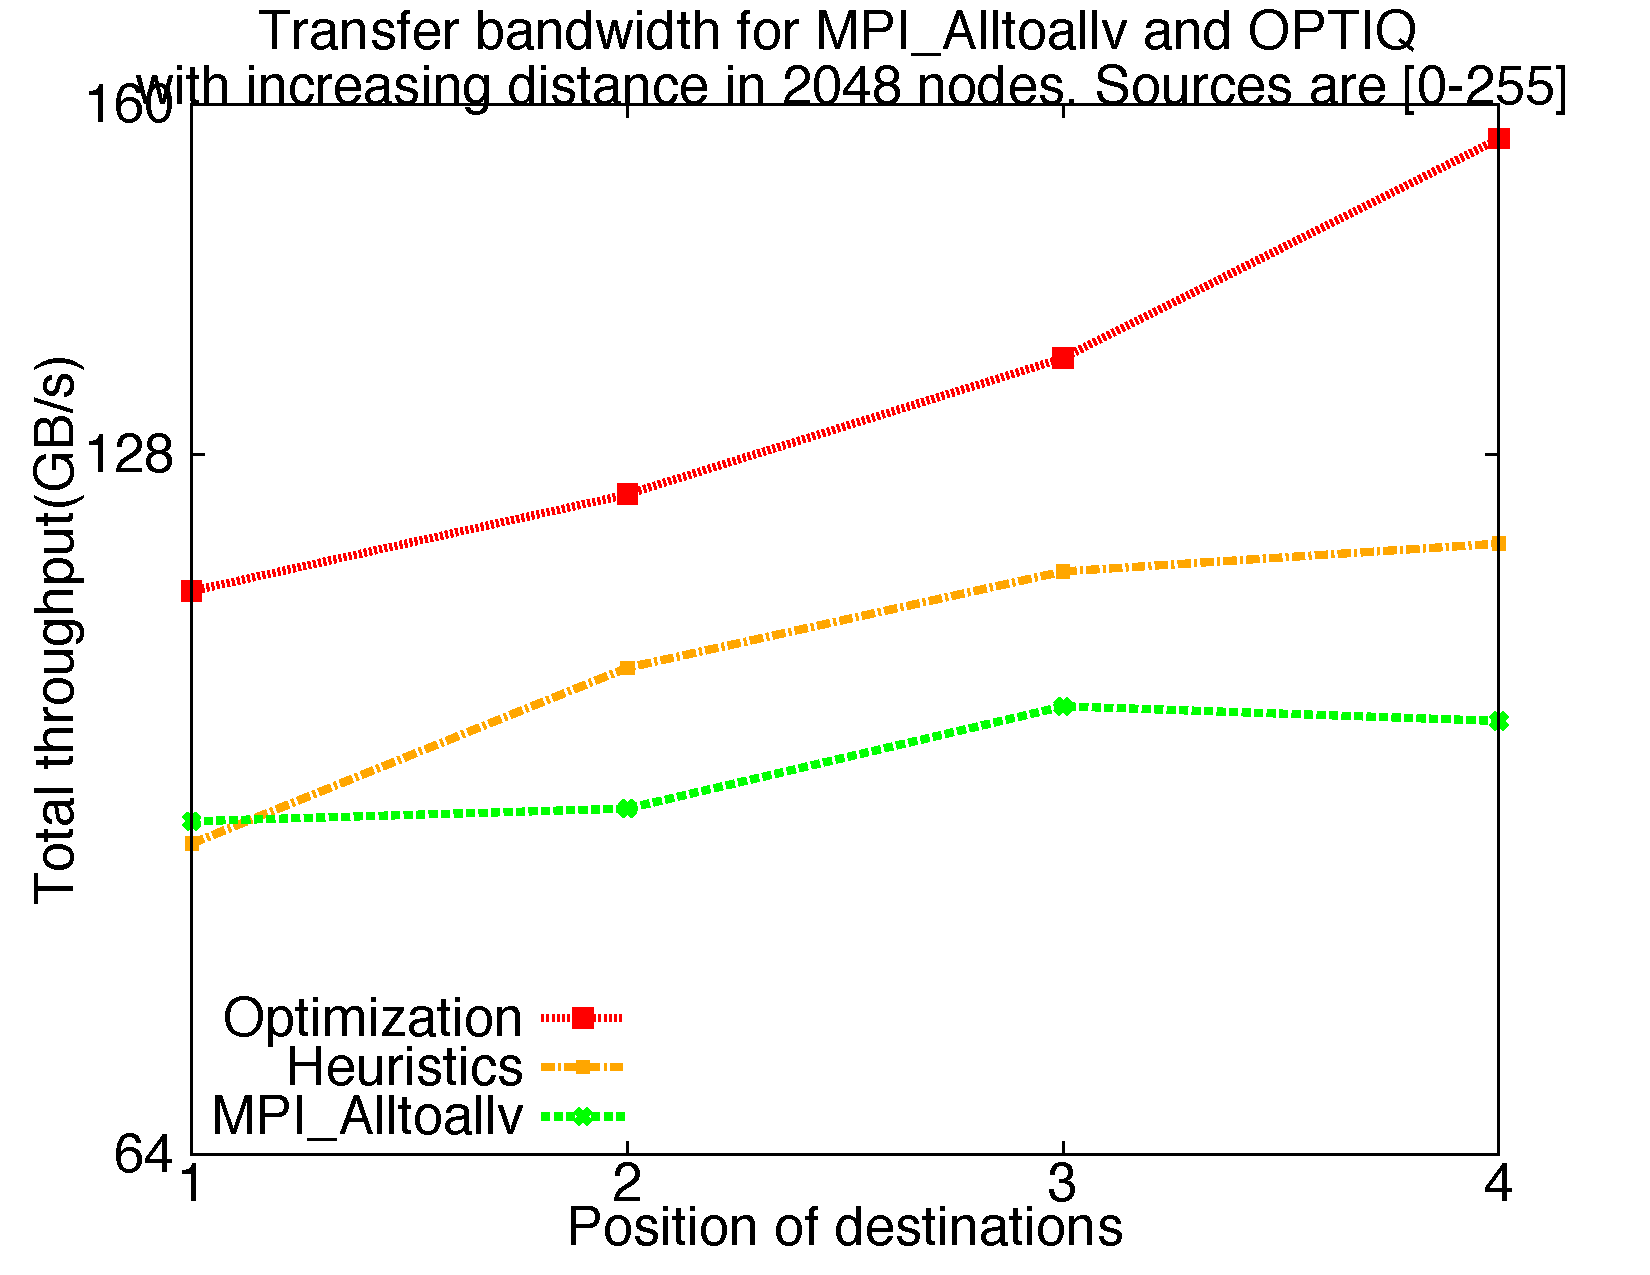
\includegraphics[width=\textwidth]{figures/incrdist_disjoint.pdf}
                \caption{Disjoint}
                \label{fig:incrdist_disjoint}
        \end{subfigure}%
        ~ %add desired spacing between images, e. g. ~, \quad, \qquad, \hfill etc.
          %(or a blank line to force the subfigure onto a new line)
        \begin{subfigure}[b]{0.32\textwidth}
                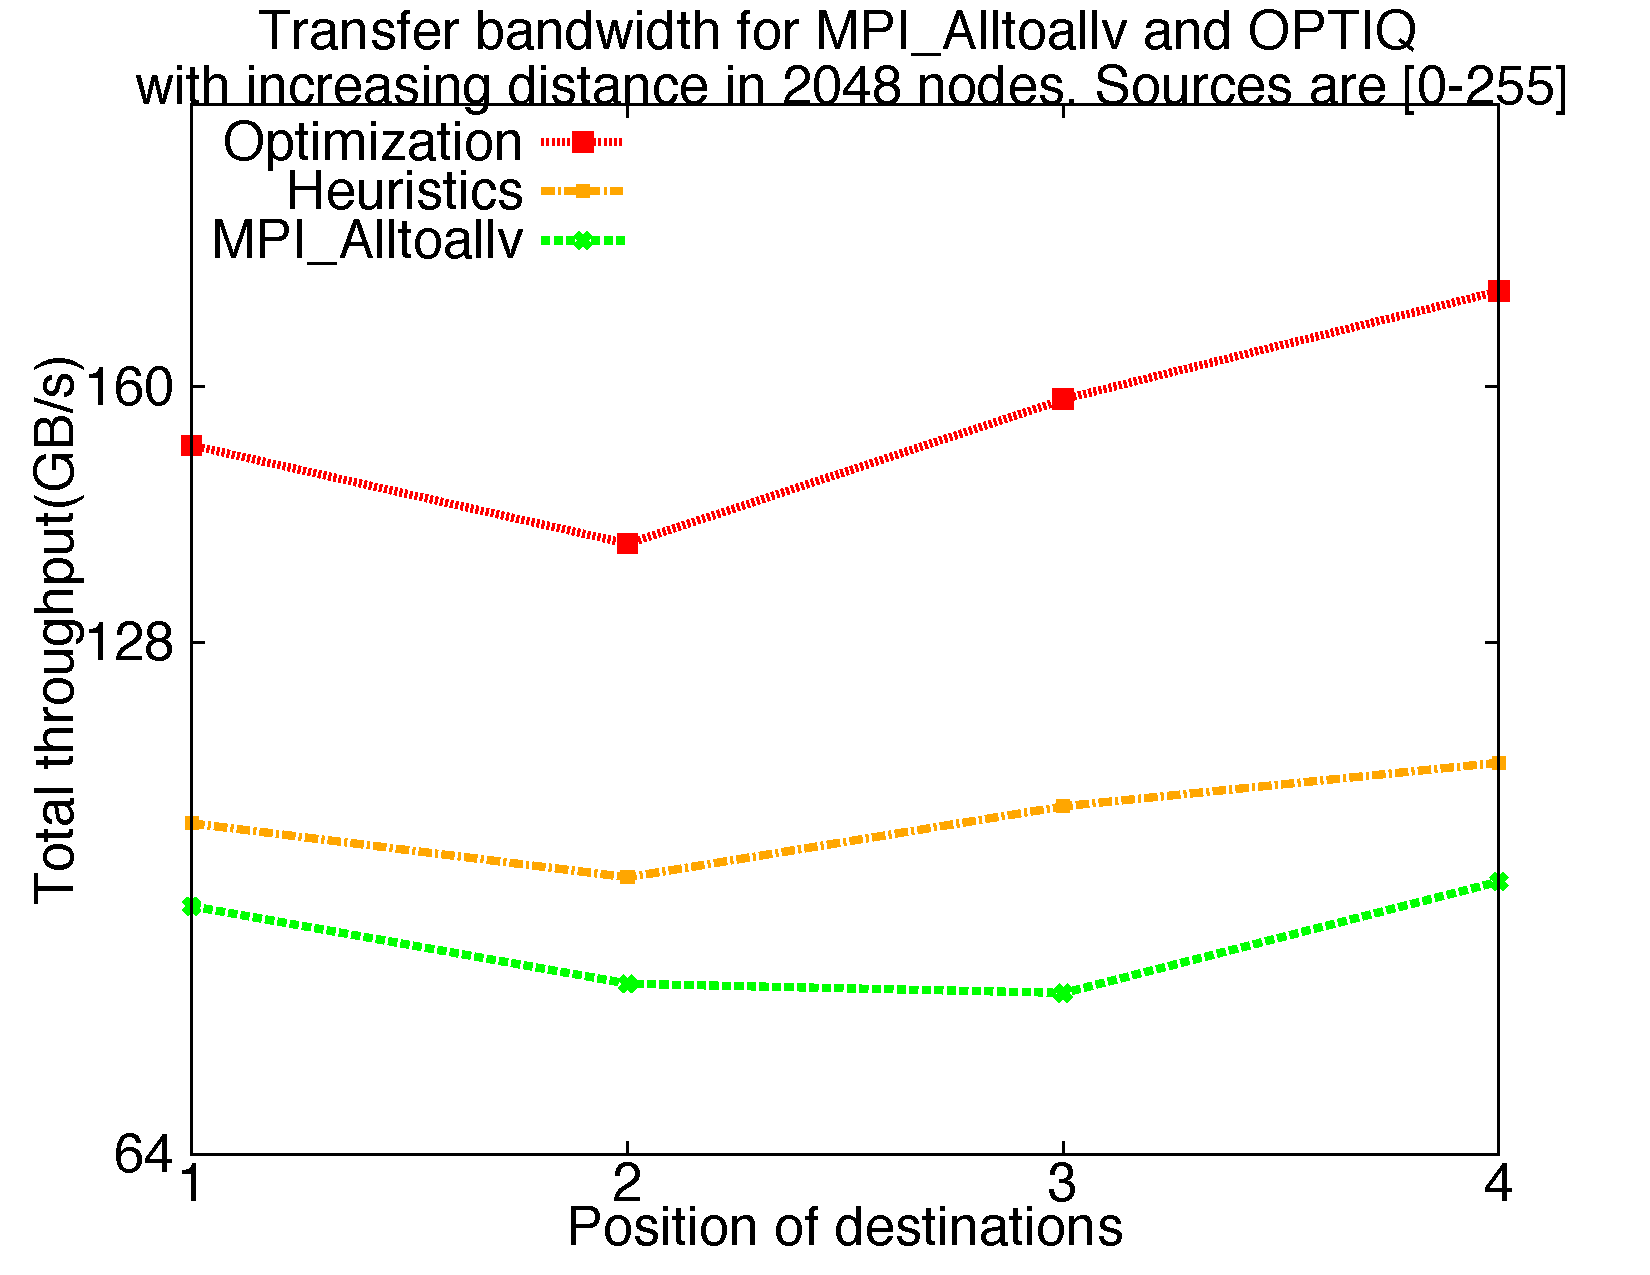
\includegraphics[width=\textwidth]{figures/incrdist_overlap}
                \caption{Overlap}
                \label{fig:incrdist_overlap}
        \end{subfigure}
        ~ %add desired spacing between images, e. g. ~, \quad, \qquad, \hfill etc.
          %(or a blank line to force the subfigure onto a new line)
        \begin{subfigure}[b]{0.32\textwidth}
                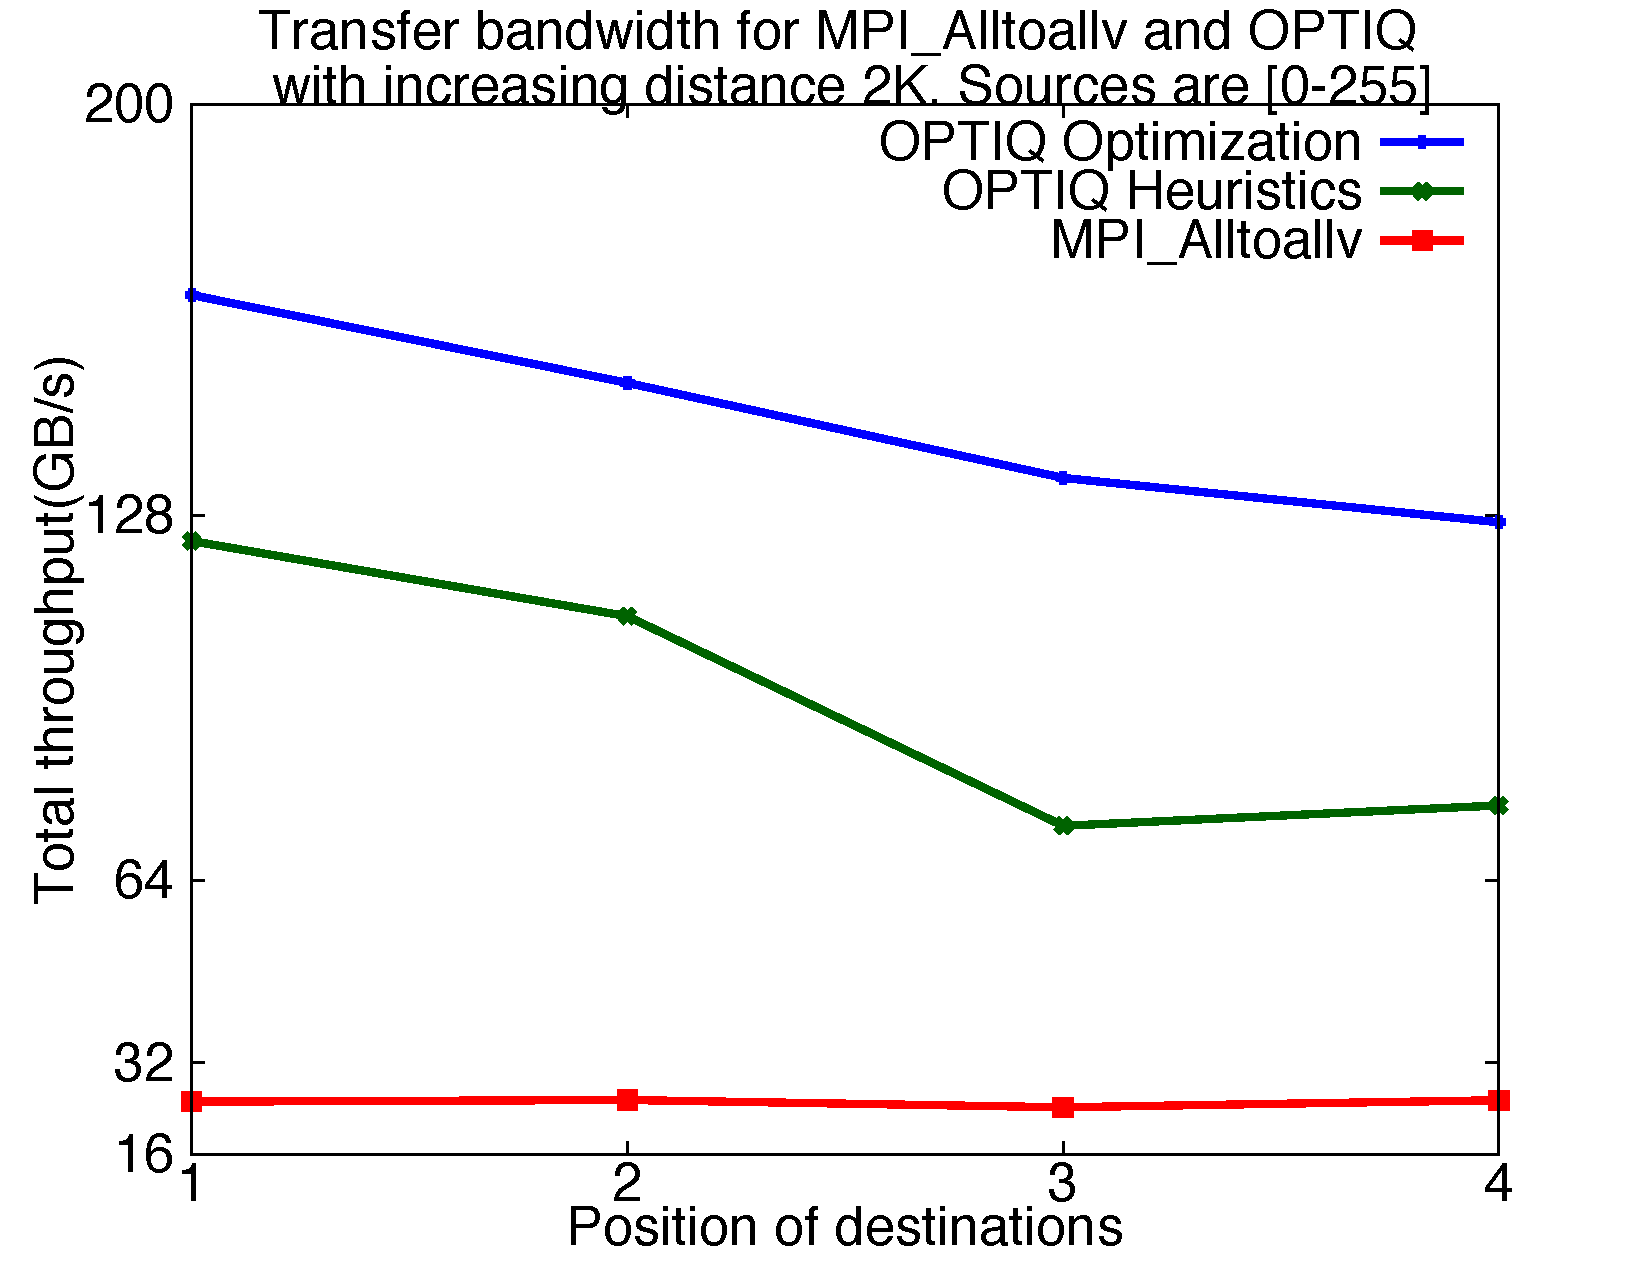
\includegraphics[width=\textwidth]{figures/incrdist_subset}
                \caption{Subset}
                \label{fig:incrdist_subset}
        \end{subfigure}
        \caption{Total data movement throughput when increasing distance between sources and destinations.}
        \label{fig:incrdist}
\end{figure*}

\begin{table*}[!htbp]
   \centering
    \begin{tabular}{| l | p{0.5cm} | p{0.5cm} | p{0.5cm} | p{0.5cm} | p{0.5cm} | p{0.5cm} |p{0.5cm} | p{0.5cm} | p{0.5cm} | p{0.5cm} |p{0.5cm} | p{0.5cm} |p{0.5cm} | p{0.5cm} |p{0.5cm} | p{0.5cm} |}
    \hline
     Positions & \multicolumn{4}{ c | }{1} & \multicolumn{4}{ c| }{2} & \multicolumn{4}{ c| }{3} & \multicolumn{4}{ c| }{4} \\ \hline
     Patterns & {Max} & Avg & Opt Paths & Heu Paths & Max & Avg & Opt Paths & Heu Paths & Max & Avg & Opt Paths & Heu Paths & Max & Avg & Opt Paths & Heu Paths \\ \hline
     Disjoint & 14 & 7.50 & 1105 & 2822 & 14  & 7.50 & 1372 & 2887 & 15 & 8.50 & 1547 & 3668 & 15 & 8.50 & 1672 & 3834 \\ \hline
     Overlap & 13 & 7.25 & 2085 & 6460 & 14  & 7.69 & 2152 & 3671 & 15 & 7.88 & 2337 & 6548 & 18 & 9.59 & 2399 & 7010 \\ \hline
     Subset &  20 & 8.56 & 1840 & 3422 & 21  & 8.56 & 1639 & 3364 & 22 & 9.06 & 1594 & 3119 & 23 & 9.06 & 1477 & 3087 \\ \hline
    \end{tabular}
    \caption{Maximum (Max) and average (Avg) distance (number of hops) and number of paths (Paths) between souces and destinations at each position.}
    \label{table:incrdist}
\end{table*}

As shown in Figure \ref{fig:incrdist}, both Optimization and Heuristcs approaches outperform MPI\_Alltoallv. 

The number of paths produced by Optimization approach are 1105 to 1372, 1547 and 1672 respectively. With increasing number of paths, the hopbytes, number of copies per paths and data load per physical link decrease, thus increasing in performance as shown in Figure \ref{fig:incrdist}. The same trend is observed in the Heuristics approach.
